\paragraph{Desarrollo técnico}
Este diseño, más simplificado, se trataba de un sistema ASK, con un receptor de conversión directa. 
La parte principal del circuito era la etapa de entrada, compuesta por un filtro de entrada sintonizable, y una etapa de amplificación de corriente formada por un par Darlington. Parte de la salida se realimentaba positivamente al filtro de entrada, aumentando la sensibilidad del receptor. La salida del par Darlington, era tratada y amplificada generando la señal de salida. 
\paragraph{}
Se muestra un esquema del receptor en la figura \ref{fig:crono_radio2} junto con la implementaci\'on real del diseño con algunas modificaciones en la figura \ref{fig:crono_radio2_real}.
\begin{figure}[h!]
    \centering
    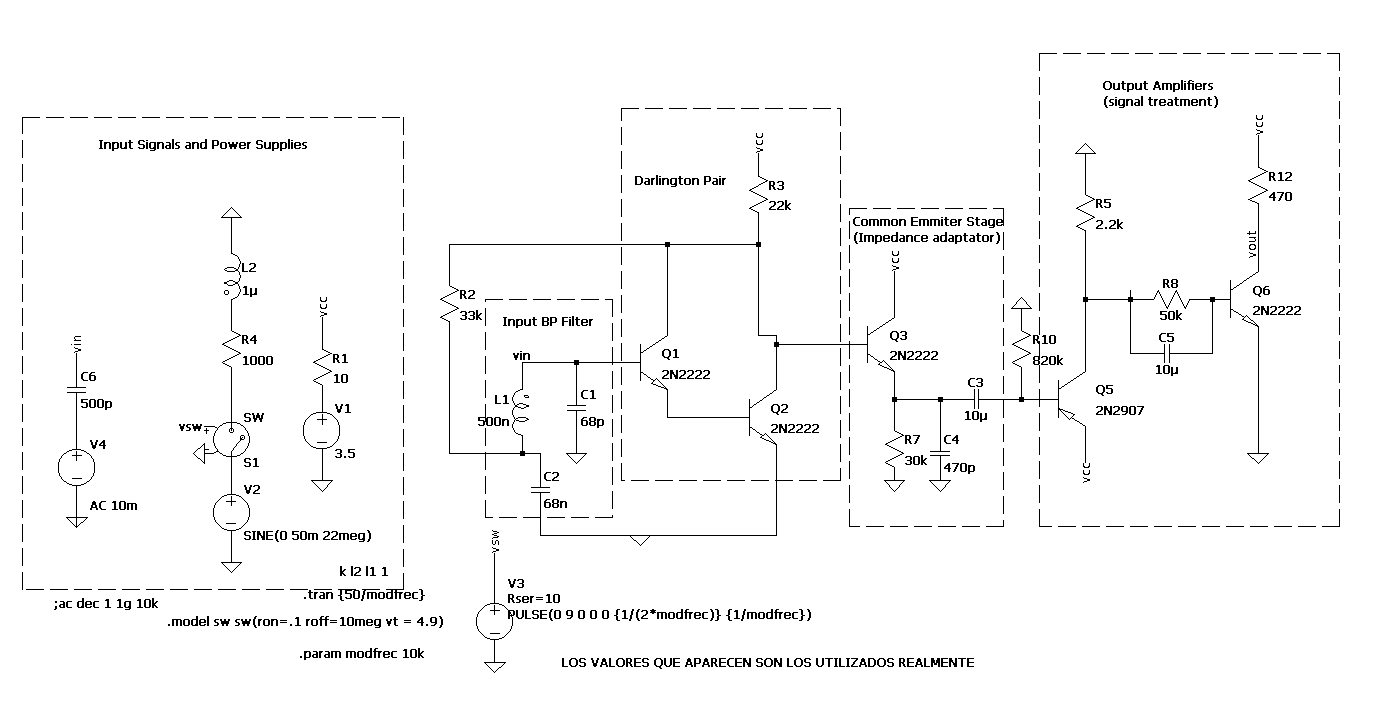
\includegraphics[scale=1, width=1\textwidth]{crono_radio2}
    \caption{sch radio2}
    \label{fig:crono_radio2}
\end{figure}

\begin{figure}[h!]
    \centering
    \includegraphics[scale=.8, width=.8\textwidth]{crono_radio2_real}
    \caption{radio2 real}
    \label{fig:crono_radio2_real}
\end{figure}

\paragraph{Motivos de reemplazo}
Este diseño tenía un objetivo principal: ser sencillo y funcional.
A pesar de conseguir una sintonización y comunicación adecuada, personalmente, no estaba suficientemente satisfecho con la distancia alcanzada. Se trató de diseñar amplificadores de RF a la entrada junto a un filtro inicial. En ese momento descubrí la dificultad de diseñar amplificadores de RF y buenos filtros. 
\paragraph{}
Otra estrategia fue la de incorporar un mezclador a la entrada. Tras varias pruebas sin obtener mejoras claras, se cambió al diseño presentado en el proyecto, un receptor super-regenerativo, el cual consigue ser funcional con muy pocos componentes.
